\newpage
\section{Validação da malha de vórtices}

Antes das análises, verificou-se que a discretização escolhida para o modelo
é suficiente. Todas as superfícies foram refinadas simultaneamente em seis
níveis, com totais de cerca de 100 a 2.000 vórtices, mantendo as proporções
entre asa e empenagens. Uma sétima malha, quatro vezes mais fina que a
adotada, foi executada apenas para servir de referência no cálculo dos
desvios. Cada nível rodou na condição do ponto de projeto, com $M = 0{,}85$
e meta de sustentação $C_L = 0{,}5053$. As métricas acompanhadas cobrem as
famílias de resultados usadas neste relatório: o ângulo de ataque de
equilíbrio, a derivada $C_{L\alpha}$, o arrasto induzido e a posição do
ponto neutro.

\begin{table}[H]
\centering
\caption{Convergência de malha na condição do ponto de projeto.}\label{tab:convergencia}
\renewcommand{\arraystretch}{1.25}
\begin{tabular}{ccccccc}
\toprule
Malha da asa & Vórtices & $\alpha$ [graus] & $C_{L\alpha}$ [1/rad] &
$C_{D,\mathrm{ind}}$ & $C_{D,\mathrm{ff}}$ (Trefftz) & $x_{np}$ [m] \\
\midrule
$3\times 12$ & 110 & 3,9041 & 6,4022 & 0,01057 & 0,00925 & 29,9379 \\
$5\times 16$ & 217 & 3,8870 & 6,4288 & 0,01063 & 0,00924 & 30,0270 \\
$8\times 25$ & 532 & 3,8741 & 6,4584 & 0,01019 & 0,00919 & 30,0547 \\
$10\times 35$ & 966 & 3,8823 & 6,4533 & 0,01022 & 0,00924 & 30,0634 \\
$12\times 40$ (adotada) & 1.312 & 3,8752 & 6,4626 & 0,01014 & 0,00923 & 30,0651 \\
$15\times 50$ & 2.050 & 3,8720 & 6,4697 & 0,01015 & 0,00922 & 30,0703 \\
$24\times 80$ (referência) & 5.248 & 3,8700 & 6,4737 & 0,00991 & 0,00923 & 30,0776 \\
\bottomrule
\end{tabular}
\end{table}

\begin{figure}[H]
\centering
\caption{Desvio percentual das métricas em relação à malha de referência
($24\times 80$), em escala logarítmica. A linha tracejada marca a malha
adotada.}\label{fig:convergencia}
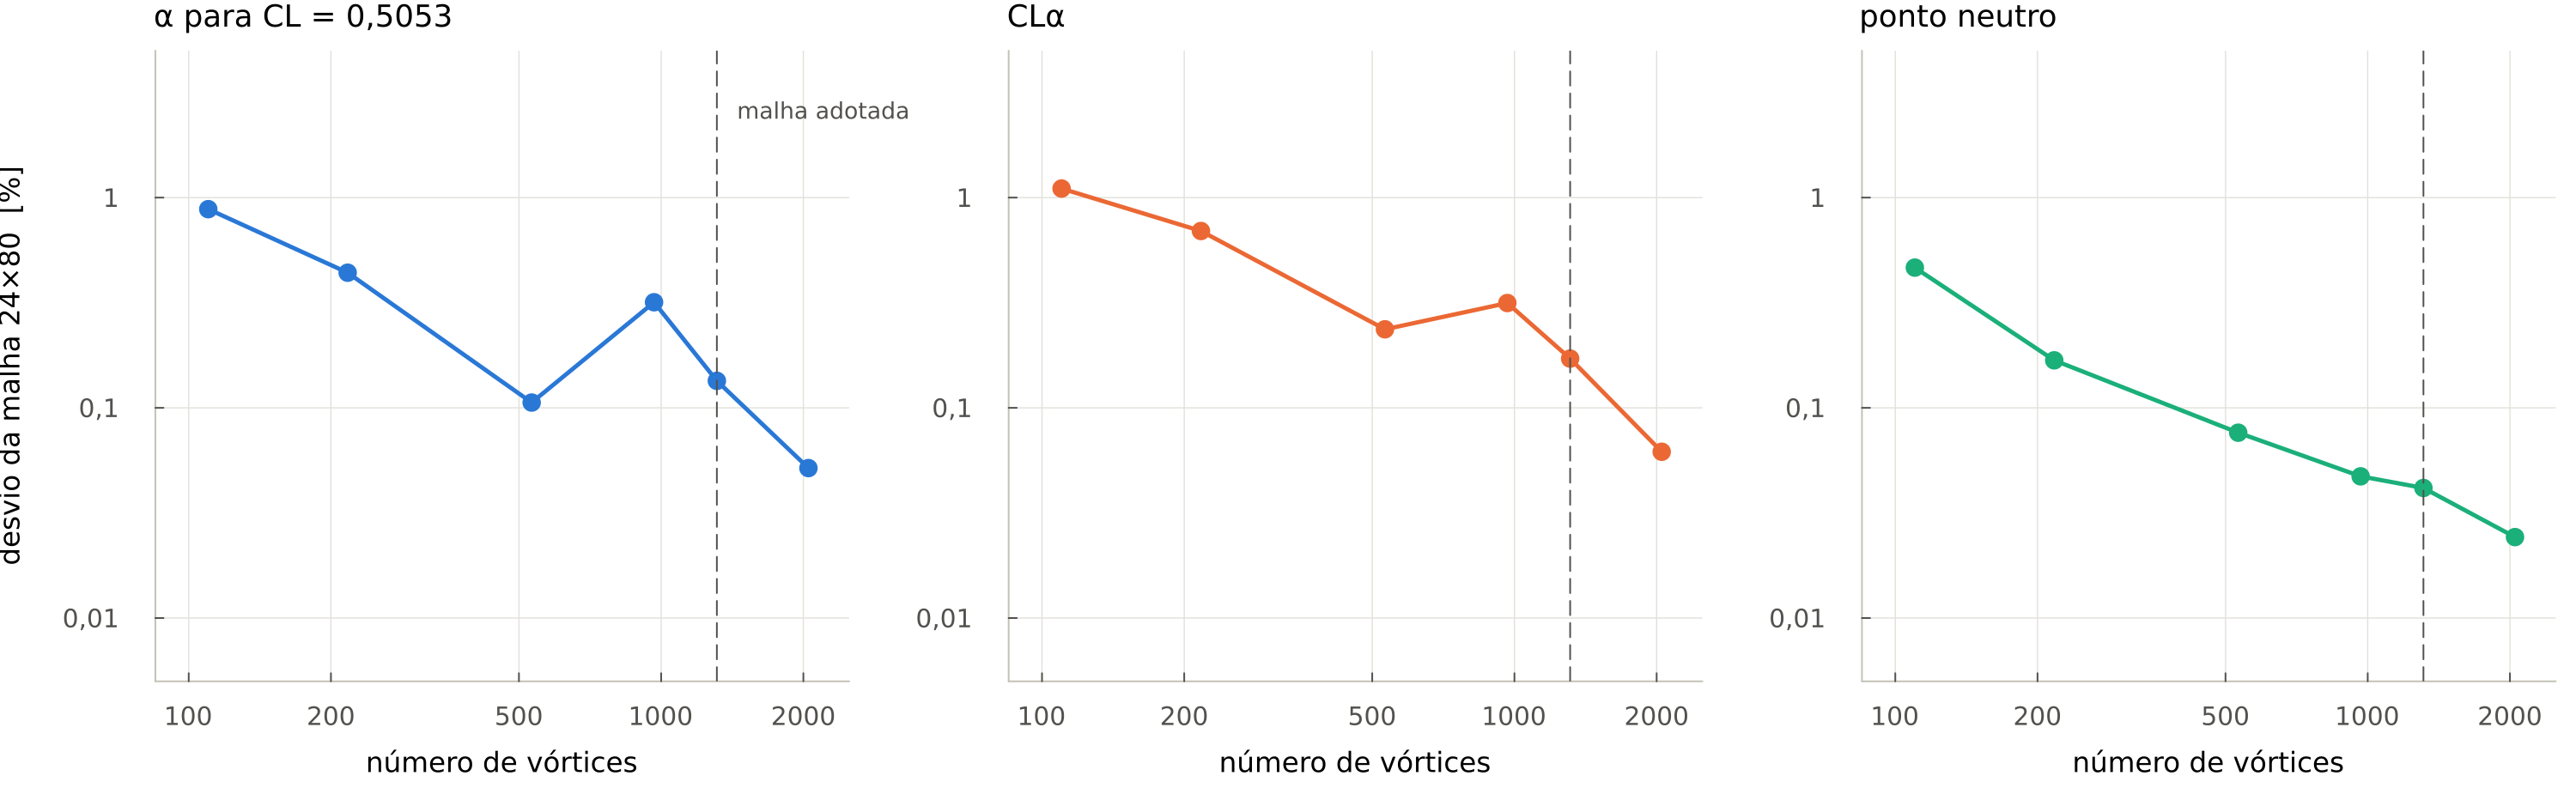
\includegraphics[width=\linewidth]{images/03_convergencia/convergencia_malha.png}
\end{figure}

A Figura~\ref{fig:convergencia} apresenta o desvio percentual em relação à
malha de referência das três métricas que exibem transiente de convergência
na faixa varrida. As três caem de forma consistente com o refino, de cerca
de 1\% na malha mais grossa para menos de 0,1\% na mais fina. Na malha
adotada, o ângulo de ataque difere da referência em 0,14\%, a derivada
$C_{L\alpha}$ em 0,17\% e o ponto neutro em 0,04\%, o que corresponde a
3,5~cm ou 0,05\,\%MAC.

O arrasto induzido do plano de Trefftz, que é a medida limpa do método, já
parte convergido: varia menos de 0,5\% em toda a varredura e a malha
adotada difere da referência em 0,01\% (Tabela~\ref{tab:convergencia}). A
integração de campo próximo oscila numa banda de cerca de 2\% sem tendência
com o refino, comportamento conhecido dessa forma de cálculo, e por isso a
curva de Trefftz é a referência para julgar o arrasto. Refinos além de
2.000 vórtices foram avaliados e os desvios apenas flutuam num piso de
ruído abaixo de 0,15\%, sem queda sistemática, o que confirma que a
varredura apresentada cobre toda a região de interesse.

A malha adotada nos arquivos da entrega, com $12\times 40$ painéis na asa e
1.312 vórtices no total, foi portanto considerada convergida para os
propósitos deste trabalho, com custo compatível com as rodadas interativas
exigidas pelo roteiro.
